\section{Nand to Tetris and the Hack Architecture} \label{hack-architecture}
Nand to Tetris is divided into several sections that can be worked on or skipped more or less independently of each other.
Each section is further removed from the actual hardware than its predecessor.
In the beginning, the students create the necessary chips and logic gates, starting with only a nand gate.
This section is not part of this thesis, but it may become relevant in future additions to the application~\ref{future-work}.
After that, students will work with assembler and create their own assembler with generated code targeting the CPU from the previous section.
The application created as part of this work contains an emulator that can run that assembly directly without further compilation.
This allows students to run their assembly code in the same application as their VM code from the later sections.
In the next section, students work closely with VM bytecode, first writing a translator from bytecode to assembly, and later writing a complete game using the high-level programming language Jack, which was designed for this course.
At the end, students will create their own compiler for said high-level language.
They will also implement a standard library for it that abstracts many of the direct interactions with the platform, such as printing text to the screen.
The last two parts are relevant to this project because students can run both the VM code and their compiled assembly in the emulator.
The main focus of this project is on the game mentioned above, which is created in Project 9.
It may seem strange to develop a whole new emulator mainly to improve a single project out of twelve, but this one exercise is the ``Tetris'' referred to in the title of the course.
Although Project 9 is not the final project, for many it is the highlight of the course.
This is illustrated by the fact that nine of the twelve examples listed under the ``Cool Stuff''~\cite{n2tweb} tab on the official website are Jack programs that would qualify as Project 9 solutions.
So if the goal is to improve the overall student experience, it makes sense to focus on this part.
Nevertheless, the emulators created as part of this thesis can also improve the experience for other projects~\ref{evaluation}.

% \subsection{The sections of Nand to Tetris}
% \begin{itemize}
%   \item Chips und Logic Gates (nicht Teil der Arbeit)
%   \item CPU und Assembly
%   \item Virtuelle Machine
%   \item High level Sprache und Betriebssystem (nicht Teil der Arbeit)
% \end{itemize}

\subsection{The operating principles of the Hack VM}
The simple C program in~\cref{lst:c-add-123} shows how one might write a loop that adds the numbers 1, 2, and 3 together.
In mathematical notation, it would be written as \(\sum_{i=1}^{3}i\).
This program may seem unremarkable at first glance, but it incorporates quite a few important concepts of modern programming languages, such as variables, loops, conditions, and arithmetic operations.
Although the program itself is trivial, its translation into machine code and subsequent execution by the computer is not.
Since machine code is highly dependent on the target architecture, the following section is specific to the Hack platform. That being said, the concepts discussed are important not only for most other VM implementations, but also for machine code generated by a C or Rust compiler.
This is especially true for the stack, which is an important concept in almost every existing programming language.

C is an imperative language, which means that we have to tell the computer how to calculate the result instead of just telling it what we want.
The program begins with the declaration of two variables called \(i\) and \(sum\).
The first is used to hold the number of iterations performed, while the second holds the final result, which is the sum of all \(i\) we iterated over.

\begin{lstlisting}[
  language=C,
  caption={A C program to calculate \(\sum_{i=1}^{3}i\).},
  label={lst:c-add-123},
  captionpos=b]
  int i = 1;
  int sum = 0;
  while (i <= 3) {
    sum += i;
    i++;
  }
\end{lstlisting}

To translate the program above into something that can be interpreted by the Hack VM, one must first understand the stack.
A stack is an abstract data structure with only two fundamental operations: Push and Pop.
The push operation adds an element to the top of the stack, while the pop operation removes the top element.
This means that the element that was pushed onto the stack last is removed first when a pop is performed.
For this reason, the stack model is called last-in-first-out (LIFO)~\cite{nisan2005}.
This model is simple but powerful and allows a very elegant description of calculations.
For example, to perform an addition, first both operands are pushed onto the stack, then the addition instruction pops these two numbers from the stack and pushes the result of the addition onto it instead.
This is illustrated in~\cref{fig:stack-add}, where 2 is pushed on top of 1 before adding both.
The stack is often represented as growing downward, but in the Hack architecture it actually grows upward, so this representation is more appropriate.

\begin{center}
  \begin{figure}[ht]
    \centering
    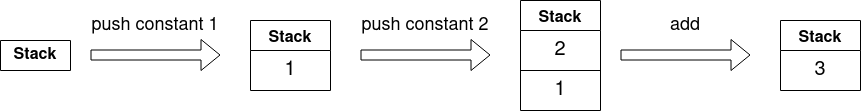
\includegraphics[width=14cm]{fig/stack-add.png}
    \caption{Adding 1 and 2 in a stack based VM.}
    \label{fig:stack-add}
  \end{figure}
\end{center}

Unlike many other architectures, push and pop in the Hack architecture can also be used to read and write arbitrary memory addresses, so no other memory-related instructions are required. For this reason, they are the only instructions in Hack that can manipulate memory outside the stack.
This is made possible by extending both instructions with a segment and an index. The segment acts as an offset that the VM adds to the index that follows it.
The address for the instruction is therefore computed as \(address=offset(segment)+index\).
It is used either as the destination where the result of a pop operation is written, or as the source location of a value to be pushed.

Only two of the eight possible segments are used in~\cref{lst:hack-bytecode}.
The local offset reads its offset from the first memory cell: \(address=RAM[1]+index\). So a ``pop local 3'' would remove the top most element of the stack and write it to \(RAM[1]+3\).
In contrast, the constant segment differs from all other segments in that it does not add anything to the index before treating the result as an address, but simply pushes the index directly onto the stack without performing a memory read.
This means that the constant segment cannot be used with the pop instruction.

With this knowledge the bytecode~\ref{lst:hack-bytecode} becomes readable.
It starts by initializing \(i\) and \(sum\) to one and zero respectively, just like the C code~\ref{lst:c-add-123}.
Afterwards, a label is declared, which is simply a position in the bytecode that can be used as a target for goto instructions.
The loop is implemented between this label and the label on the last line and can be divided into three parts.
The first part performs the exit condition check to determine if the loop body should be executed.
To do this, it first puts the value of \(i\) on the stack and then jumps out of the loop if \(\neg(i < 4)\), which is equivalent to \(i > 3\).
If the aforementioned check was false, the loop body is executed.
This means that the actual implementation of a loop condition works the other way around than in the C example, where we enter the loop if the condition was true.
This inversion is done because the code does not perform a jump when the loop is executed.
Since most loops are run more than once, this saves a lot of jumps in the program flow, which are often quite expensive.
To update \(sum\), the VM loads the current value of \(sum\) onto the stack, then the current value of \(i\), and after adding the two, the result is written back to \(sum\).
Updating \(i\) works basically the same way, but with a constant value of one instead of another local variable being added.
Then we simply jump back to the beginning of the loop, where the next check for the exit condition is performed, and continue this process until that condition is met.

\subsection{Hack Bytecode} \label{hack-bytecode}
\begin{lstlisting}[
  language=Hack,
  caption={A Hack VM program to calculate \(\sum_{i=1}^{3}i\).},
  label={lst:hack-bytecode},
  captionpos=b]
  // i = 1
  push constant 1
  pop local 0

  // sum = 0
  push constant 0
  pop local 1

  label LOOP_START

  // the Hack bytecode does not have an <= instruction,
  // therefore use i < 4 instead of i <= 3
  // if i >= 4 jump out of the loop
  push local 0
  push constant 4
  lt
  not
  if-goto LOOP_END

  // sum = sum + i
  push local 1
  push local 0
  add
  pop local 1

  // i = i + 1
  push local 0
  push constant 1
  add
  pop local 0

  // jump to the beginning of the loop again
  goto LOOP_START
  label LOOP_END
\end{lstlisting}
